
%% bare_conf.tex
%% V1.3
%% 2007/01/11
%% by Michael Shell
%% See:
%% http://www.michaelshell.org/
%% for current contact information.
%%
%% This is a skeleton file demonstrating the use of IEEEtran.cls
%% (requires IEEEtran.cls version 1.7 or later) with an IEEE conference paper.
%%
%% Support sites:
%% http://www.michaelshell.org/tex/ieeetran/
%% http://www.ctan.org/tex-archive/macros/latex/contrib/IEEEtran/
%% and
%% http://www.ieee.org/

%%*************************************************************************
%% Legal Notice:
%% This code is offered as-is without any warranty either expressed or
%% implied; without even the implied warranty of MERCHANTABILITY or
%% FITNESS FOR A PARTICULAR PURPOSE! 
%% User assumes all risk.
%% In no event shall IEEE or any contributor to this code be liable for
%% any damages or losses, including, but not limited to, incidental,
%% consequential, or any other damages, resulting from the use or misuse
%% of any information contained here.
%%
%% All comments are the opinions of their respective authors and are not
%% necessarily endorsed by the IEEE.
%%
%% This work is distributed under the LaTeX Project Public License (LPPL)
%% ( http://www.latex-project.org/ ) version 1.3, and may be freely used,
%% distributed and modified. A copy of the LPPL, version 1.3, is included
%% in the base LaTeX documentation of all distributions of LaTeX released
%% 2003/12/01 or later.
%% Retain all contribution notices and credits.
%% ** Modified files should be clearly indicated as such, including  **
%% ** renaming them and changing author support contact information. **
%%
%% File list of work: IEEEtran.cls, IEEEtran_HOWTO.pdf, bare_adv.tex,
%%                    bare_conf.tex, bare_jrnl.tex, bare_jrnl_compsoc.tex
%%*************************************************************************

% *** Authors should verify (and, if needed, correct) their LaTeX system  ***
% *** with the testflow diagnostic prior to trusting their LaTeX platform ***
% *** with production work. IEEE's font choices can trigger bugs that do  ***
% *** not appear when using other class files.                            ***
% The testflow support page is at:
% http://www.michaelshell.org/tex/testflow/



% Note that the a4paper option is mainly intended so that authors in
% countries using A4 can easily print to A4 and see how their papers will
% look in print - the typesetting of the document will not typically be
% affected with changes in paper size (but the bottom and side margins will).
% Use the testflow package mentioned above to verify correct handling of
% both paper sizes by the user's LaTeX system.
%
% Also note that the "draftcls" or "draftclsnofoot", not "draft", option
% should be used if it is desired that the figures are to be displayed in
% draft mode.
%
\documentclass[conference, twocolumn, oneside, 10pt]{IEEEtran}
% Add the compsoc option for Computer Society conferences.
%
% If IEEEtran.cls has not been installed into the LaTeX system files,
% manually specify the path to it like:
% \documentclass[conference]{../sty/IEEEtran}





% Some very useful LaTeX packages include:
% (uncomment the ones you want to load)


% *** MISC UTILITY PACKAGES ***
%
%\usepackage{ifpdf}
% Heiko Oberdiek's ifpdf.sty is very useful if you need conditional
% compilation based on whether the output is pdf or dvi.
% usage:
% \ifpdf
%   % pdf code
% \else
%   % dvi code
% \fi
% The latest version of ifpdf.sty can be obtained from:
% http://www.ctan.org/tex-archive/macros/latex/contrib/oberdiek/
% Also, note that IEEEtran.cls V1.7 and later provides a builtin
% \ifCLASSINFOpdf conditional that works the same way.
% When switching from latex to pdflatex and vice-versa, the compiler may
% have to be run twice to clear warning/error messages.






% *** CITATION PACKAGES ***
%
\usepackage{cite}
% cite.sty was written by Donald Arseneau
% V1.6 and later of IEEEtran pre-defines the format of the cite.sty package
% \cite{} output to follow that of IEEE. Loading the cite package will
% result in citation numbers being automatically sorted and properly
% "compressed/ranged". e.g., [1], [9], [2], [7], [5], [6] without using
% cite.sty will become [1], [2], [5]--[7], [9] using cite.sty. cite.sty's
% \cite will automatically add leading space, if needed. Use cite.sty's
% noadjust option (cite.sty V3.8 and later) if you want to turn this off.
% cite.sty is already installed on most LaTeX systems. Be sure and use
% version 4.0 (2003-05-27) and later if using hyperref.sty. cite.sty does
% not currently provide for hyperlinked citations.
% The latest version can be obtained at:
% http://www.ctan.org/tex-archive/macros/latex/contrib/cite/
% The documentation is contained in the cite.sty file itself.






% *** GRAPHICS RELATED PACKAGES ***
%
\ifCLASSINFOpdf
  \usepackage[pdftex]{graphicx}
  % declare the path(s) where your graphic files are
  % \graphicspath{{../pdf/}{../jpeg/}}
  % and their extensions so you won't have to specify these with
  % every instance of \includegraphics
  % \DeclareGraphicsExtensions{.pdf,.jpeg,.png}
\else
  % or other class option (dvipsone, dvipdf, if not using dvips). graphicx
  % will default to the driver specified in the system graphics.cfg if no
  % driver is specified.
  \usepackage[dvips]{graphicx}
  % declare the path(s) where your graphic files are
  % \graphicspath{{../eps/}}
  % and their extensions so you won't have to specify these with
  % every instance of \includegraphics
  % \DeclareGraphicsExtensions{.eps}
\fi
% graphicx was written by David Carlisle and Sebastian Rahtz. It is
% required if you want graphics, photos, etc. graphicx.sty is already
% installed on most LaTeX systems. The latest version and documentation can
% be obtained at: 
% http://www.ctan.org/tex-archive/macros/latex/required/graphics/
% Another good source of documentation is "Using Imported Graphics in
% LaTeX2e" by Keith Reckdahl which can be found as epslatex.ps or
% epslatex.pdf at: http://www.ctan.org/tex-archive/info/
%
% latex, and pdflatex in dvi mode, support graphics in encapsulated
% postscript (.eps) format. pdflatex in pdf mode supports graphics
% in .pdf, .jpeg, .png and .mps (metapost) formats. Users should ensure
% that all non-photo figures use a vector format (.eps, .pdf, .mps) and
% not a bitmapped formats (.jpeg, .png). IEEE frowns on bitmapped formats
% which can result in "jaggedy"/blurry rendering of lines and letters as
% well as large increases in file sizes.
%
% You can find documentation about the pdfTeX application at:
% http://www.tug.org/applications/pdftex





% *** MATH PACKAGES ***
%
\usepackage[cmex10]{amsmath}
% A popular package from the American Mathematical Society that provides
% many useful and powerful commands for dealing with mathematics. If using
% it, be sure to load this package with the cmex10 option to ensure that
% only type 1 fonts will utilized at all point sizes. Without this option,
% it is possible that some math symbols, particularly those within
% footnotes, will be rendered in bitmap form which will result in a
% document that can not be IEEE Xplore compliant!
%
% Also, note that the amsmath package sets \interdisplaylinepenalty to 10000
% thus preventing page breaks from occurring within multiline equations. Use:
%\interdisplaylinepenalty=2500
% after loading amsmath to restore such page breaks as IEEEtran.cls normally
% does. amsmath.sty is already installed on most LaTeX systems. The latest
% version and documentation can be obtained at:
% http://www.ctan.org/tex-archive/macros/latex/required/amslatex/math/





% *** SPECIALIZED LIST PACKAGES ***
%
\usepackage{algorithm}
\usepackage{algorithmic}
% algorithmic.sty was written by Peter Williams and Rogerio Brito.
% This package provides an algorithmic environment fo describing algorithms.
% You can use the algorithmic environment in-text or within a figure
% environment to provide for a floating algorithm. Do NOT use the algorithm
% floating environment provided by algorithm.sty (by the same authors) or
% algorithm2e.sty (by Christophe Fiorio) as IEEE does not use dedicated
% algorithm float types and packages that provide these will not provide
% correct IEEE style captions. The latest version and documentation of
% algorithmic.sty can be obtained at:
% http://www.ctan.org/tex-archive/macros/latex/contrib/algorithms/
% There is also a support site at:
% http://algorithms.berlios.de/index.html
% Also of interest may be the (relatively newer and more customizable)
% algorithmicx.sty package by Szasz Janos:
% http://www.ctan.org/tex-archive/macros/latex/contrib/algorithmicx/




% *** ALIGNMENT PACKAGES ***
%
\usepackage{array}
% Frank Mittelbach's and David Carlisle's array.sty patches and improves
% the standard LaTeX2e array and tabular environments to provide better
% appearance and additional user controls. As the default LaTeX2e table
% generation code is lacking to the point of almost being broken with
% respect to the quality of the end results, all users are strongly
% advised to use an enhanced (at the very least that provided by array.sty)
% set of table tools. array.sty is already installed on most systems. The
% latest version and documentation can be obtained at:
% http://www.ctan.org/tex-archive/macros/latex/required/tools/


%\usepackage{mdwmath}
%\usepackage{mdwtab}
% Also highly recommended is Mark Wooding's extremely powerful MDW tools,
% especially mdwmath.sty and mdwtab.sty which are used to format equations
% and tables, respectively. The MDWtools set is already installed on most
% LaTeX systems. The lastest version and documentation is available at:
% http://www.ctan.org/tex-archive/macros/latex/contrib/mdwtools/


% IEEEtran contains the IEEEeqnarray family of commands that can be used to
% generate multiline equations as well as matrices, tables, etc., of high
% quality.


%\usepackage{eqparbox}
% Also of notable interest is Scott Pakin's eqparbox package for creating
% (automatically sized) equal width boxes - aka "natural width parboxes".
% Available at:
% http://www.ctan.org/tex-archive/macros/latex/contrib/eqparbox/





% *** SUBFIGURE PACKAGES ***
\usepackage[tight,footnotesize]{subfigure}
% subfigure.sty was written by Steven Douglas Cochran. This package makes it
% easy to put subfigures in your figures. e.g., "Figure 1a and 1b". For IEEE
% work, it is a good idea to load it with the tight package option to reduce
% the amount of white space around the subfigures. subfigure.sty is already
% installed on most LaTeX systems. The latest version and documentation can
% be obtained at:
% http://www.ctan.org/tex-archive/obsolete/macros/latex/contrib/subfigure/
% subfigure.sty has been superceeded by subfig.sty.



% \usepackage[caption=false]{caption}
% \usepackage[font=footnotesize]{subfig}
% subfig.sty, also written by Steven Douglas Cochran, is the modern
% replacement for subfigure.sty. However, subfig.sty requires and
% automatically loads Axel Sommerfeldt's caption.sty which will override
% IEEEtran.cls handling of captions and this will result in nonIEEE style
% figure/table captions. To prevent this problem, be sure and preload
% caption.sty with its "caption=false" package option. This is will preserve
% IEEEtran.cls handing of captions. Version 1.3 (2005/06/28) and later 
% (recommended due to many improvements over 1.2) of subfig.sty supports
% the caption=false option directly:
%\usepackage[caption=false,font=footnotesize]{subfig}
%
% The latest version and documentation can be obtained at:
% http://www.ctan.org/tex-archive/macros/latex/contrib/subfig/
% The latest version and documentation of caption.sty can be obtained at:
% http://www.ctan.org/tex-archive/macros/latex/contrib/caption/




% *** FLOAT PACKAGES ***
%
%\usepackage{fixltx2e}
% fixltx2e, the successor to the earlier fix2col.sty, was written by
% Frank Mittelbach and David Carlisle. This package corrects a few problems
% in the LaTeX2e kernel, the most notable of which is that in current
% LaTeX2e releases, the ordering of single and double column floats is not
% guaranteed to be preserved. Thus, an unpatched LaTeX2e can allow a
% single column figure to be placed prior to an earlier double column
% figure. The latest version and documentation can be found at:
% http://www.ctan.org/tex-archive/macros/latex/base/



%\usepackage{stfloats}
% stfloats.sty was written by Sigitas Tolusis. This package gives LaTeX2e
% the ability to do double column floats at the bottom of the page as well
% as the top. (e.g., "\begin{figure*}[!b]" is not normally possible in
% LaTeX2e). It also provides a command:
%\fnbelowfloat
% to enable the placement of footnotes below bottom floats (the standard
% LaTeX2e kernel puts them above bottom floats). This is an invasive package
% which rewrites many portions of the LaTeX2e float routines. It may not work
% with other packages that modify the LaTeX2e float routines. The latest
% version and documentation can be obtained at:
% http://www.ctan.org/tex-archive/macros/latex/contrib/sttools/
% Documentation is contained in the stfloats.sty comments as well as in the
% presfull.pdf file. Do not use the stfloats baselinefloat ability as IEEE
% does not allow \baselineskip to stretch. Authors submitting work to the
% IEEE should note that IEEE rarely uses double column equations and
% that authors should try to avoid such use. Do not be tempted to use the
% cuted.sty or midfloat.sty packages (also by Sigitas Tolusis) as IEEE does
% not format its papers in such ways.





% *** PDF, URL AND HYPERLINK PACKAGES ***
%
%\usepackage{url}
% url.sty was written by Donald Arseneau. It provides better support for
% handling and breaking URLs. url.sty is already installed on most LaTeX
% systems. The latest version can be obtained at:
% http://www.ctan.org/tex-archive/macros/latex/contrib/misc/
% Read the url.sty source comments for usage information. Basically,
% \url{my_url_here}.





% *** Do not adjust lengths that control margins, column widths, etc. ***
% *** Do not use packages that alter fonts (such as pslatex).         ***
% There should be no need to do such things with IEEEtran.cls V1.6 and later.
% (Unless specifically asked to do so by the journal or conference you plan
% to submit to, of course. )


% correct bad hyphenation here
\hyphenation{op-tical net-works semi-conduc-tor}


\begin{document}
%
% paper title
% can use linebreaks \\ within to get better formatting as desired
\title{Network Failure Analysis for CENIC}


% author names and affiliations
% use a multiple column layout for up to three different
% affiliations
\author{
\IEEEauthorblockN{ }
\and
\IEEEauthorblockN{ }
\and
\IEEEauthorblockN{ }
}

%\author{\IEEEauthorblockN{Michael Shell}
%\IEEEauthorblockA{School of Electrical and\\Computer Engineering\\
%Georgia Institute of Technology\\
%Atlanta, Georgia 30332--0250\\
%Email: http://www.michaelshell.org/contact.html}
%\and
%\IEEEauthorblockN{Homer Simpson}
%\IEEEauthorblockA{Twentieth Century Fox\\
%Springfield, USA\\
%Email: homer@thesimpsons.com}
%\and
%\IEEEauthorblockN{James Kirk\\ and Montgomery Scott}
%\IEEEauthorblockA{Starfleet Academy\\
%San Francisco, California 96678-2391\\
%Telephone: (800) 555--1212\\
%Fax: (888) 555--1212}}

% conference papers do not typically use \thanks and this command
% is locked out in conference mode. If really needed, such as for
% the acknowledgment of grants, issue a \IEEEoverridecommandlockouts
% after \documentclass

% for over three affiliations, or if they all won't fit within the width
% of the page, use this alternative format:
% 
%\author{\IEEEauthorblockN{Michael Shell\IEEEauthorrefmark{1},
%Homer Simpson\IEEEauthorrefmark{2},
%James Kirk\IEEEauthorrefmark{3}, 
%Montgomery Scott\IEEEauthorrefmark{3} and
%Eldon Tyrell\IEEEauthorrefmark{4}}
%\IEEEauthorblockA{\IEEEauthorrefmark{1}School of Electrical and Computer Engineering\\
%Georgia Institute of Technology,
%Atlanta, Georgia 30332--0250\\ Email: see http://www.michaelshell.org/contact.html}
%\IEEEauthorblockA{\IEEEauthorrefmark{2}Twentieth Century Fox, Springfield, USA\\
%Email: homer@thesimpsons.com}
%\IEEEauthorblockA{\IEEEauthorrefmark{3}Starfleet Academy, San Francisco, California 96678-2391\\
%Telephone: (800) 555--1212, Fax: (888) 555--1212}
%\IEEEauthorblockA{\IEEEauthorrefmark{4}Tyrell Inc., 123 Replicant Street, Los Angeles, California 90210--4321}}




% use for special paper notices
%\IEEEspecialpapernotice{(Invited Paper)}




% make the title area
\maketitle
\thispagestyle{plain}
\pagestyle{plain}

\begin{abstract}
%\boldmath

\end{abstract}
% IEEEtran.cls defaults to using nonbold math in the Abstract.
% This preserves the distinction between vectors and scalars. However,
% if the conference you are submitting to favors bold math in the abstract,
% then you can use LaTeX's standard command \boldmath at the very start
% of the abstract to achieve this. Many IEEE journals/conferences frown on
% math in the abstract anyway.

% no keywords




% For peer review papers, you can put extra information on the cover
% page as needed:
% \ifCLASSOPTIONpeerreview
% \begin{center} \bfseries EDICS Category: 3-BBND \end{center}
% \fi
%
% For peerreview papers, this IEEEtran command inserts a page break and
% creates the second title. It will be ignored for other modes.
\IEEEpeerreviewmaketitle

\section{Introduction}
\label{sec:sec1}

As more and more enterprises heavily rely on the networks, there is clearly an increase in importance to provide better availability or even uninterrupted service more aggressively. However, it brings us a much challenging work to deliver such promise as we are building much more complex and larger networks comparing to years ago. Although tons of research projects have been trying to work it out, it is still not very well solved. As well as many previous work shown \cite{labovitz1999experimental, markopoulou2008characterization, padmanabhan2006study}, we believe the better analysis of the network failures should be considerably helpful for us to understand how the failures occur, how they affect the network behaviors and how to eliminate them in order to provide better availability.

To deliver such network failure analysis in practice, one will need much information about the causes, time lasted, influence to the network and many other specifics that are clearly not intuitively provided by the network protocols in use currently. Thus, the traditional approaches \cite{paxson1997end, cunha2011predicting} for doing this kind of analysis is to build some extra software or hardware support, which would incur large amount of expense and perhaps performance overhead. Consequently, most of such failure analysis are performed in the research community. To our knowledge, California Fault Lines \cite{turner2010california} is the first piece of work that trying to extract these information from commonly used production networks today.

Other than reconstructing historical network failure events, we are able to perform further characterization and analysis on those failures with very similar "cheap and dirty" data which we can easily obtain from today's networks. To better understand the network behavior, we describe and validate a methodology to map the routing changes to corresponding ISIS failures. In addition, we propose an approach to better understand how the failures occur and how they affect the network behaviors. Furthermore, characterization and discussion are presented about the unexpected network behaviors including routing loops and non-existent links.

Specifically, we set up six source machines respectively at UC Berkeley, UC San Diego, UC Los Angeles, UC Santa Barbara, UC Davis and UC Santa Cruz, all in CENIC (the Corporation for Education Network Initiatives in California) which is the autonomous system we are trying to analyze. Each of the six machines are supposed to send a series of traceroute requests to the end hosts of the failing link when it is detected with the help of syslog messages automatically sent by CENIC. Firstly, we map the traceroute data back to corresponding network failures for further study, and validate how well the failure detection and traceroute are working based on the mapping. Secondly, we detect the routing loops and non-existent links in the traceroute data, and carry out some statistics and characterization on these unexpected network behaviors as well as the ISIS failures. At last, with the help of link weights of CENIC, we evaluate how well the network protocols work on routing and analyze how the failures affect the network behaviors.

The rest of the paper is organized as follows. We begin with the discussion of related work in Section \ref{sec:sec2}. Then the data we use in this work is introduced in Section \ref{sec:sec3}. Section \ref{sec:sec4} presents the our methodology for the characterization and analysis, and they are validated in Section \ref{sec:sec5}. We present our analysis in Section \ref{sec:sec6} and conclude in Section \ref{sec:sec7}.

\section{Related work}
\label{sec:sec2}

bla bla

\section{Data sources}
\label{sec:sec3}

bla bla

\section{Methodology}
\label{sec:sec4}

\subsection{}

how to reconstruct the network failure history

\subsection{}

how to map the failure with traceroute

\subsection{}

loop and non-existent link detection

\section{Validation}
\label{sec:sec5}

\subsection{Network History}

Assuming the active probing of the certain network could give us a complete history of it, we had this history of the CENIC from 10/20/2012 to 02/09/2013. There were 40074 ISIS failures during this period in total.

\begin{figure}[h!]
\centering
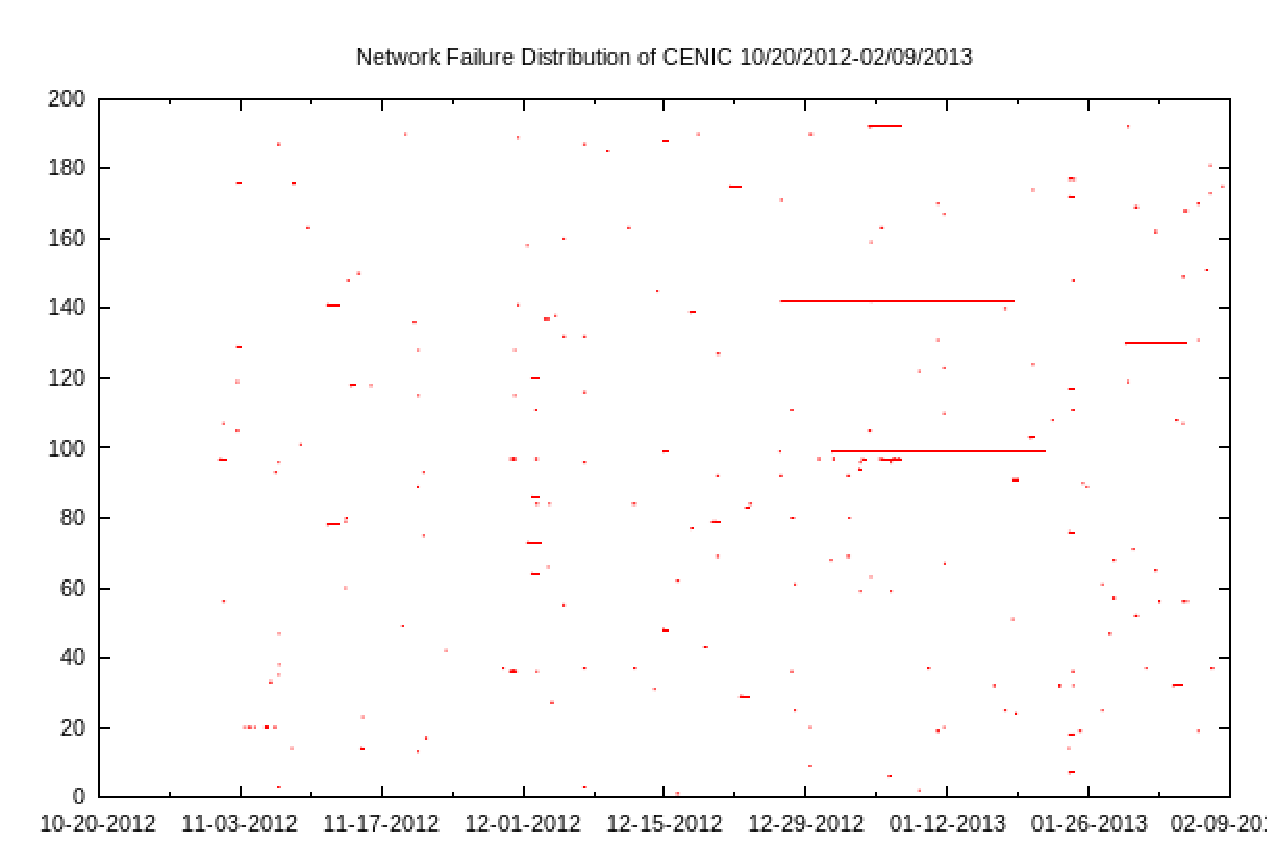
\includegraphics[scale=0.4]{plot/failure_plot.eps}
\caption{Network failures distribution of CENIC from 10/20/2012 to 02/09/2013, where Y-axis is the failure link. Most of the failures lasted for a fairly short time period and there were 192 links had failed at least once during this time period.}
\label{fig:failureplot}
\end{figure}

Since we would like to do a comparison among the route before, during and after the failure to better understand how failure affects the network behaviors, it was useful to find out how long each failure last for. Thus, the CDF of failure recovery time was shown in Figure \ref{fig:failuretime}. Surprisingly, there were 77.87\% of the failures that were recovered in 0 seconds, which means they didn't actually affect the network in the granularity of second that we used. And more than 95\% failures were recovered within 6 seconds, which could potentially make the corresponding traceroutes much less interesting. 

\begin{figure}[h!]
\centering
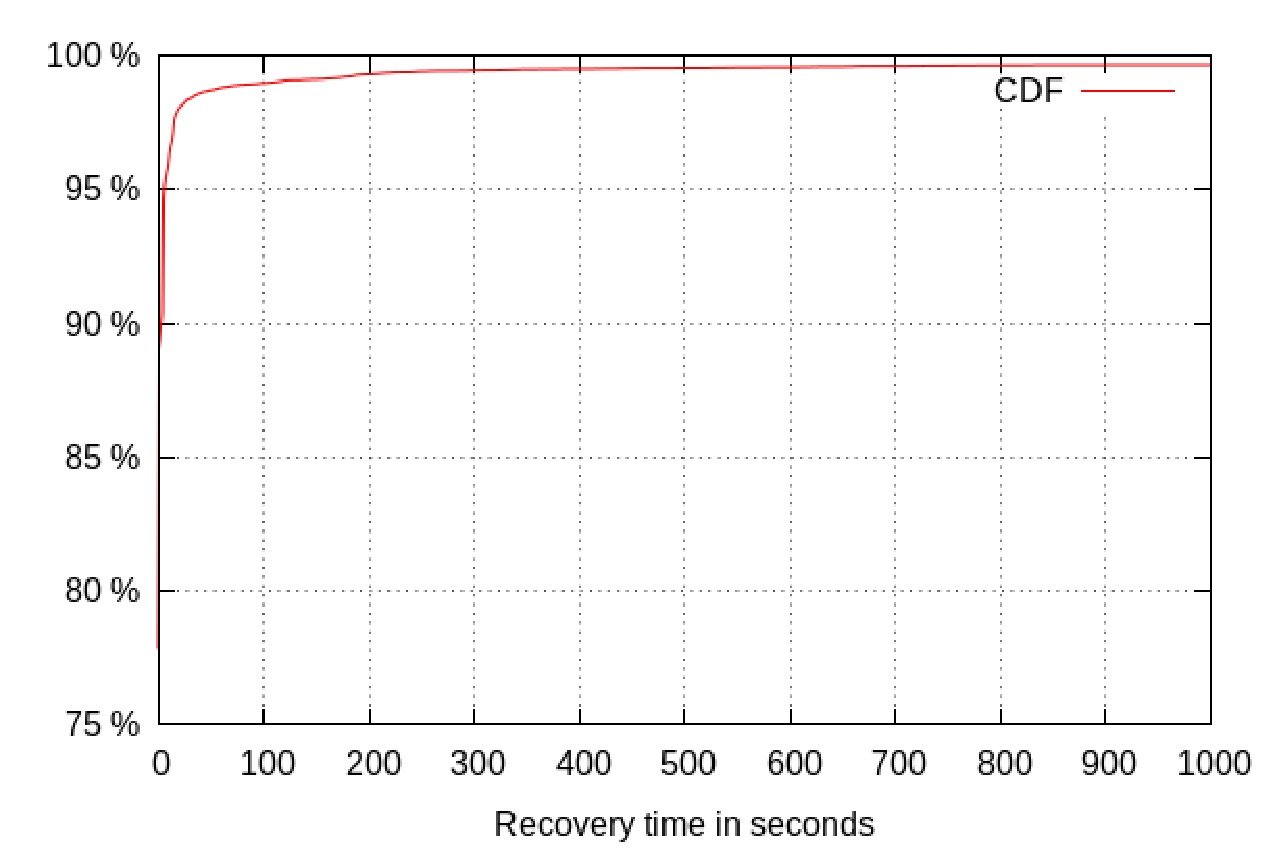
\includegraphics[scale=0.4]{plot/failure_time.eps}
\caption{Network failure recovery time CDF of CENIC where more than 95\% failures recovered within 6 seconds.}
\label{fig:failuretime}
\end{figure}

Because of the relatively short recovery time, it is very likely that the failure had already recovered before we sent very few traceroutes. Thus it could reduce the amount of data we were interested in because most of the traceroute would not even aware of the route changes due to the large granularity. However, even with small percentages, we didn't get very tiny numbers in the following analysis because of the fairly large number of failures we had in total.

\subsection{Network History Reconstruction}

To validate the network history we reconstructed from the traceroute data, we tried to map the probed failures to corresponding traceroutes. Based on the link and router map of CENIC we had successfully mapped 40073 ISIS failures to corresponding traceroute data out of the total 40074. The only one that had not been mapped was because we didn't have the IP address of the link. Thus, we believed it is save to say our failure detection works pretty well from this point.

For these 40073 detected failures, we had pinged at least one end of the failure link. And for 39505 out of 40073 (98.58\%) failures, we had pinged both ends at least once. Consequently, we believed our data is very representative for our analysis.

\subsection{Statistices of Unexpected Network Behavior (Loops \& Non-existent Links)}
In the 70831 traceroute records, we found 366 records that contain loops in total. We categorized these 366 records by the length of loop and found that more than 95\% (350 out of 366) of loops are jumping between only two routers. As of the long loop records, most of them would also fall into a two-router trap finally.
\newline


\begin{figure}[h!]
\centering
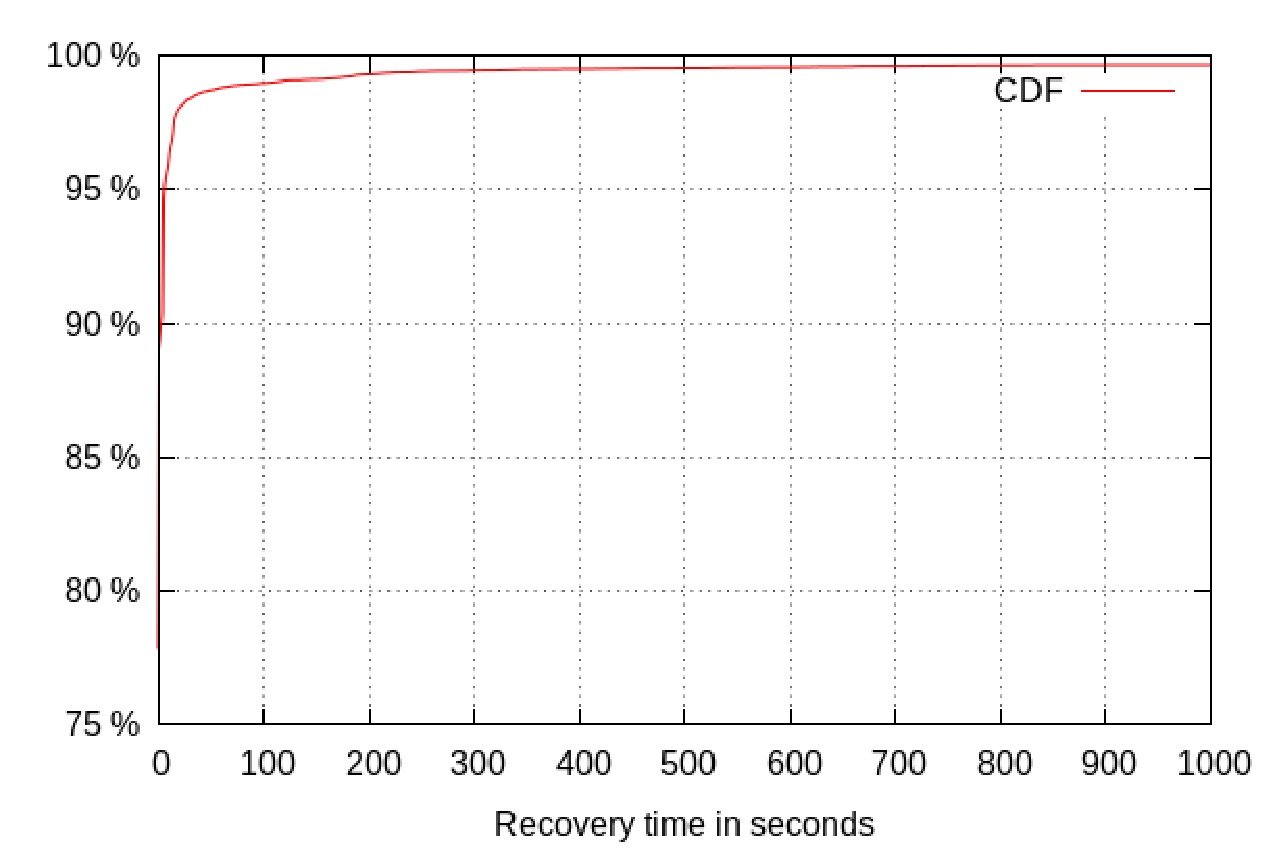
\includegraphics[scale=0.4]{plot/failure_time.eps}
\caption{Loop Length Statistics}
\label{fig:asdf}
\end{figure}

\subsection{Measurement Bias}

First of all, the granularity of the network failures and the traceroute data could potentially affect our analysis of the network behaviors. As discussed ealier, the ISIS failures were probed at the granularity of one second, while many of them lasted less than couple seconds actually. This reduced the number of interesting traceroutes since they could not even reflect the effects of such short failures. We believed that a much finer granularity of the failures would be very helpful for further analysis.

Additionally, our failure detection mechanism is based on adjacency status reported by the underlying routing protocol. For example, to ensure connectivity, the IS-IS protocol requires routers to send and
receive hello messages. By default, a router sends a hello message once every ten seconds and declares a link disconnected if no hello message is received for thirty seconds. Consequently, the failure detection could have up to 30 seconds of delay, which could reduce the accuracy of the mapping between the failure and corresponding traceroutes. In addition, this would probably affect our analysis about how the failures affected the network behaviors.

\section{Data Analysis}
\label{sec:sec6}

\subsection{Loop Characterization}

Given the traceroute data, we can figure out 


\subsection{Non-Existent Links Charaterization}

Among the 70831 trace-route records, there were 80 records has non-existent links
in them. 
%Notice that, although these 80 records only involves 44 physical links
%between routers, we didn't pay much attention on how many times they occur.
%Because, duplicate appearance in these 80 records indicate such missing links 
We classify these records into 5 categories, with respect to the complexity of
their cause. They are: normal route shift, complex route shift, shortcut,
trapped in loop, cannot verify. \\
\textbf{Normal Route Shift}\\
Consider a trace-route with max hops 5. In most situation, a certain route won't
change during the process of trace-route. However, it is possible for router to
choose another path during this process. An example is shown in figure:
\ref{fig:NormalRouteShift}.\\
\begin{figure}[h!]
\centering
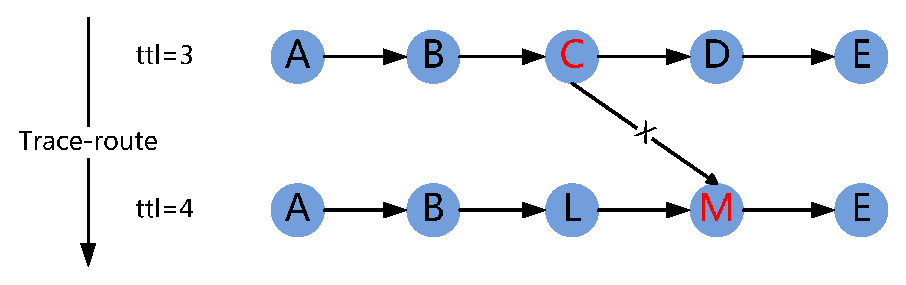
\includegraphics[scale=0.5]{plot/RouteShift.eps}
\caption{A Normal Route Shift example}
\label{fig:NormalRouteShift}
\end{figure}\\
It is important to notice in figure:\ref{fig:NormalRouteShift} that, both of the
two routes reached destination $E$, with $C$ on the third hop and $M$ on the fourth
hop. We identify this kind of links by finding valid route with the same node on
the same hop. 45 out of the 80 records fall into this category.\\
\textbf{Complex Route Shift}\\
This was a more complicated situation than in the first case. There were three
key differences with the first category. First, a complex route
shift may shift among more than 2 routes in a trace-route. Second, the picked route
is allowed to be a route that did not reach the destination.
Third, it is possible that none of other trace-route record can match a node on
a certain hop of a complex route shift. Still, consider a
trace-route with max hops 5. An example is shown in figure:
\ref{fig:ComplexRouteShift}.\\
\begin{figure}[h!]
\centering
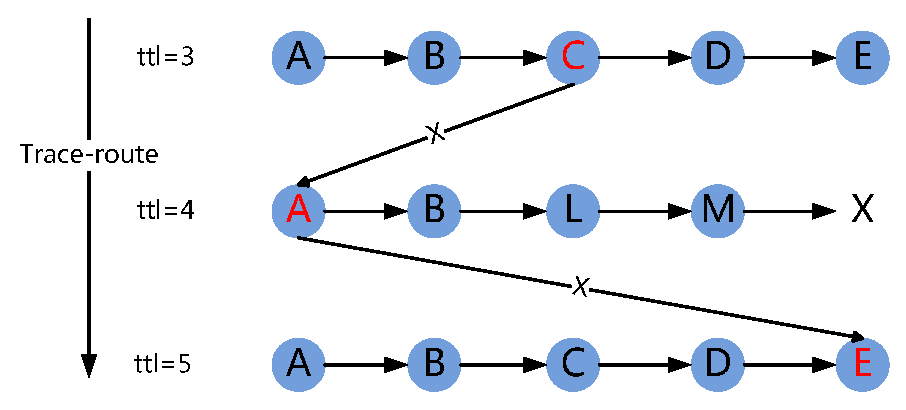
\includegraphics[scale=0.5]{plot/ComplexRouteShift.eps}
\caption{A Complex Route Shift example}
\label{fig:ComplexRouteShift}
\end{figure}\\
From figure:\ref{fig:ComplexRouteShift}, we cannot tell what exactly happened.
Although we see node $B$ on hop 4, can see no $B$ on hop 4 from any other
record. This means, we have no idea of how and why trace-route reached B on the
fourth hop. Hop 5 behaves similar with normal route shift. There were 9 records
fall into this category.\\
\textbf{Shortcut}\\
Short cut is a special case of a normal route shift, with one of the route in
the shift to be an invalid route. An example is shown in
figure:\ref{fig:Shortcut}.\\
\begin{figure}[h!]
\centering
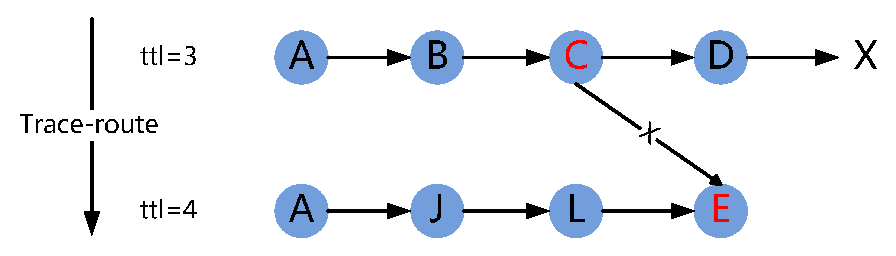
\includegraphics[scale=0.5]{plot/Shortcut.eps}
\caption{A Shortcut example}
\label{fig:Shortcut}
\end{figure}\\
To explain this phenomenon in a more intuitive way, suppose one of the router is
down, trace-route cannot get to the destination due to the router failure. Then,
during the trace-route, the router is fixed and back to work, trace-route got
the destination directly on the next hop. There were 3 records fall into this
category.\\
\textbf{Trapped in loop}\\
This is another special case of normal route shift, with one of the route is a
loopy route. An example is shown in figure:\ref{fig:TrappedInLoop}.\\
\begin{figure}[h!]
\centering
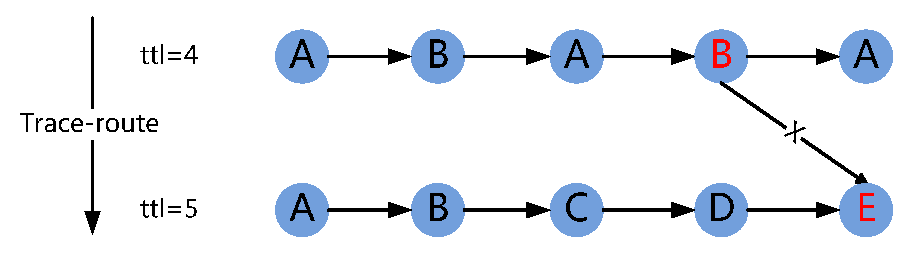
\includegraphics[scale=0.5]{plot/TrappedInLoop.eps}
\caption{Route Trapped in Loop example}
\label{fig:TrappedInLoop}
\end{figure}\\
There were 15 records fall into this category.
\textbf{Cannot verify}\\
The rest 8 records fall into this category. For these records, there exist some
node that is never seen in other trace-route records with the same source and
destination. Thus, there is no way we can tell what happened with such
records.\\ 



\subsection{Failure Analysis}

Given the traceroute data, we were able to take a closer look at the ISIS failures, which could potentially help us better understand the network behaviors and then try to reduce the number of failures. From all the 40073 failures we've ever pinged, only 125 (3.11\%) of them had ever caused a route change from at least one source. This was a relatively small number comparing with the total failures we detected, which I thought is mainly because we only had 6 sources to send traceroute requests and there are only 3 of them worked as we expected, as well as most of the failures lasted for very short time period. It would be considerably helpful if we could have more sources sending traceroute to the failure end hosts, which would probably give us more interesting routing changes.

And about half of these changes, 63 out of 125 (50.40\%), were not detectable because we could only get more or less unrecognized hops displayed as ** from traceroute. Since we couldn't recognize them, we didn't have their route weights and were not able to draw any conclusions on how their routes change quantitatively. But we could still do some analysis about the accessibility of the failure ends.

\begin{figure}[h!]
\centering
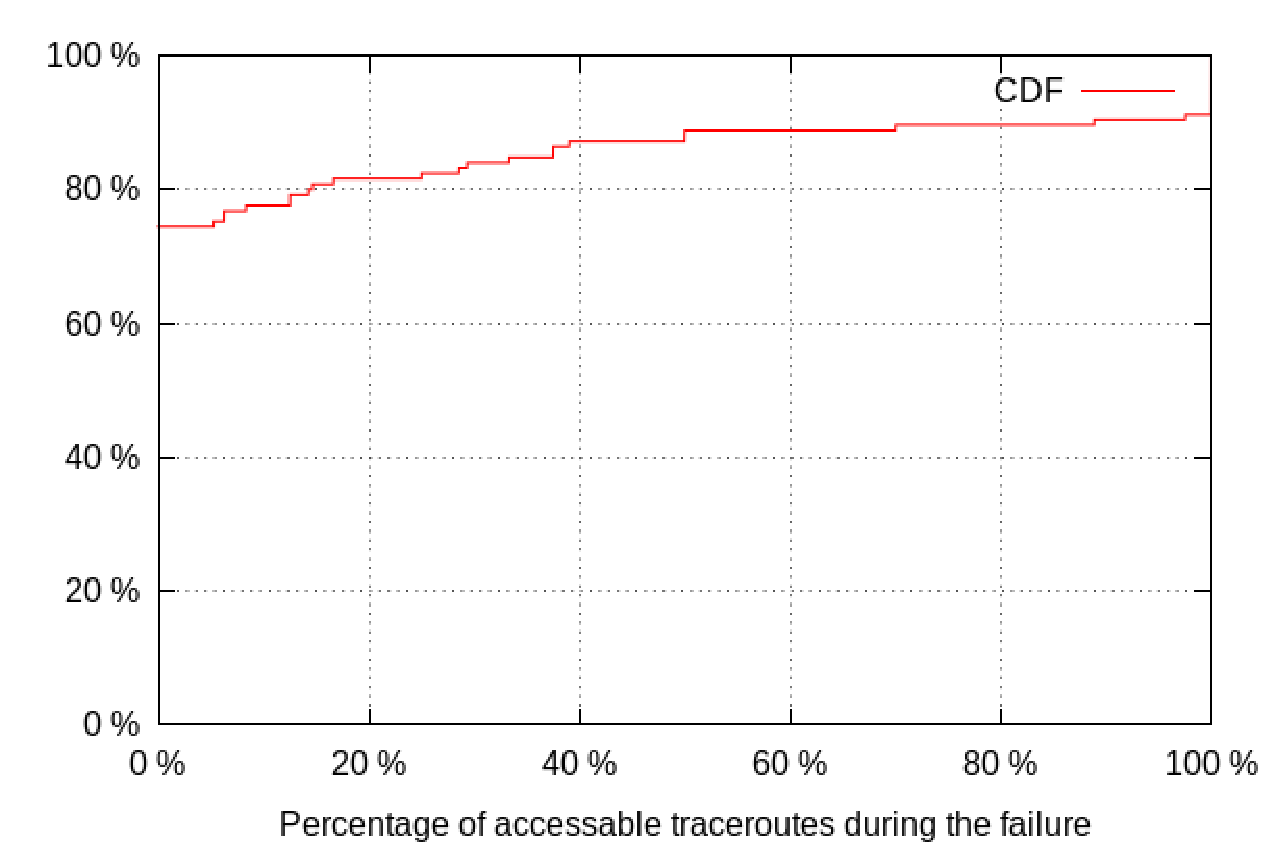
\includegraphics[scale=0.4]{plot/accessibility.eps}
\caption{Percentage CDF of accessible pings during the link failure time. 74.40\% of the 125 failures which had caused route changes hadn't affected the accessibility of the end hosts, which meant the routing protocaol worked pretty well during those failures.}
\label{fig:accessibility}
\end{figure}

It was clear in Figure \ref{fig:accessibility}, that the end hosts of 93 out of 125 (74.40\%) failures have kept reachable during the failure period. Because all these 125 failures had caused route changes, which is to say that all these routes were affected by the failures somehow, it was relatively well that the routing protocols were performing. However, there were still 8.80\% of the failures caused some of the end hosts unreachable during the whole failure period.

Furthermore, we did some statistics for the failure links, where a few links (192) occurred large number of failures (40073). From Figure \ref{fig:distribution}, we could easily find that most of the failure links had small numbers of failures ever occurred. But the most surprising part of this figure is that there are some links that had more than thousands of failures during this period of time, which were supposed to be taken care of after tens of frequent occurrences.

\begin{figure}[h!]
\centering
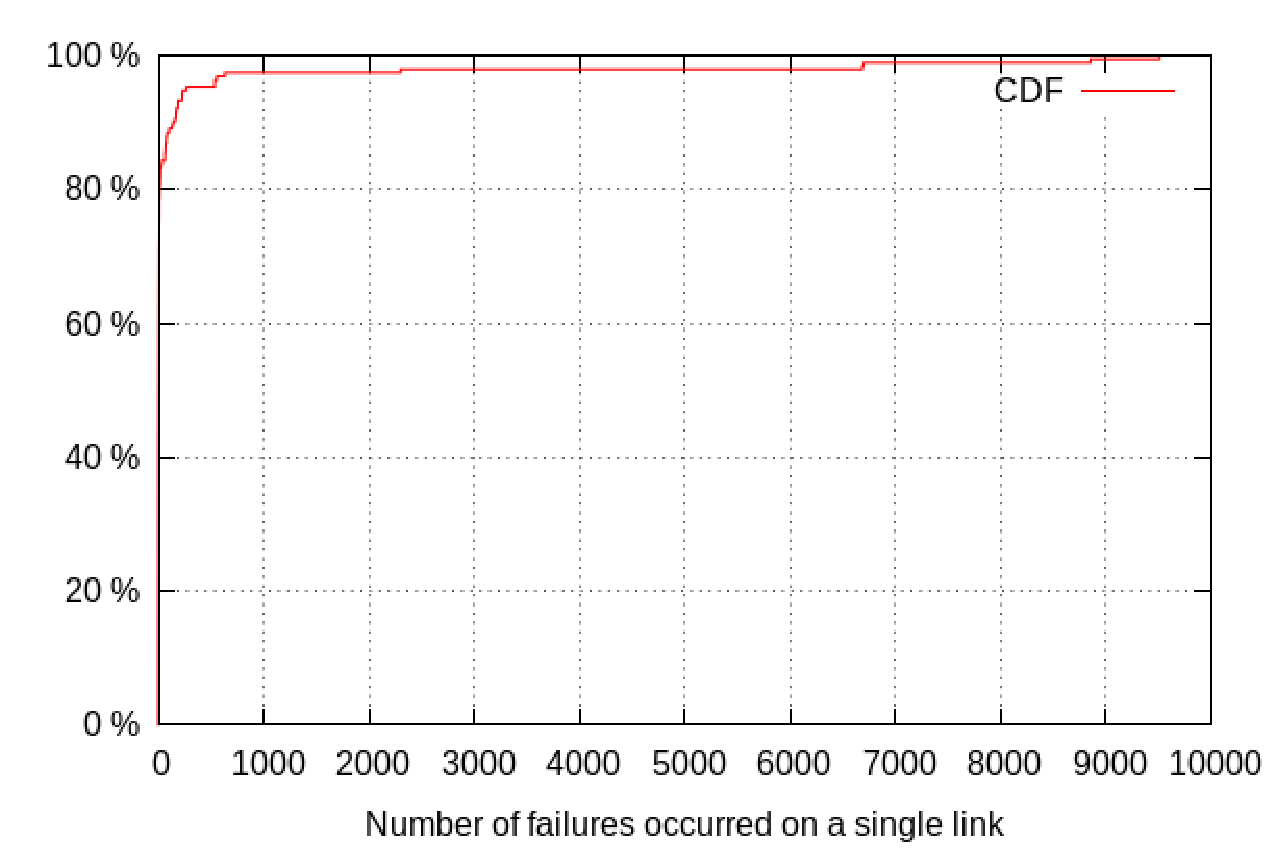
\includegraphics[scale=0.4]{plot/failure_distribution.eps}
\caption{The distribution CDF of the failure links. Most of the failure links had very small numbers of failures, where 74.48\% of them had occurred less or equal 10 failures. However, there are some links had very frequent failures that were more than 8000 times during this period.}
\label{fig:distribution}
\end{figure}

\subsection{}

routing performance characterization

\subsection{}

* how failure affects routing (better be extended into several sections)

\section{Conclusion}
\label{sec:sec7}



% conference papers do not normally have an appendix

% use section* for acknowledgment
\section*{Acknowledgment}
We thank Professor Scott Baden for his awesome lecture notes for CSE 260, and the usage of Bang HPC Cluster where we did our experiments. Also, we thank the University of Tennessee of Knoxville for the Basic Linear Algebra Subprograms.


% trigger a \newpage just before the given reference
% number - used to balance the columns on the last page
% adjust value as needed - may need to be readjusted if
% the document is modified later
%\IEEEtriggeratref{8}
% The "triggered" command can be changed if desired:
%\IEEEtriggercmd{\enlargethispage{-5in}}

% references section

% can use a bibliography generated by BibTeX as a .bbl file
% BibTeX documentation can be easily obtained at:
% http://www.ctan.org/tex-archive/biblio/bibtex/contrib/doc/
% The IEEEtran BibTeX style support page is at:
% http://www.michaelshell.org/tex/ieeetran/bibtex/
%\bibliographystyle{IEEEtran}
% argument is your BibTeX string definitions and bibliography database(s)
%\bibliography{IEEEabrv,../bib/paper}
%
% <OR> manually copy in the resultant .bbl file
% set second argument of \begin to the number of references
% (used to reserve space for the reference number labels box)
\bibliography{main}{}
\bibliographystyle{plain}

% that's all folks
\end{document}
